\section{Risikoanalyse}
\begin{figure}[H]
	\centering
	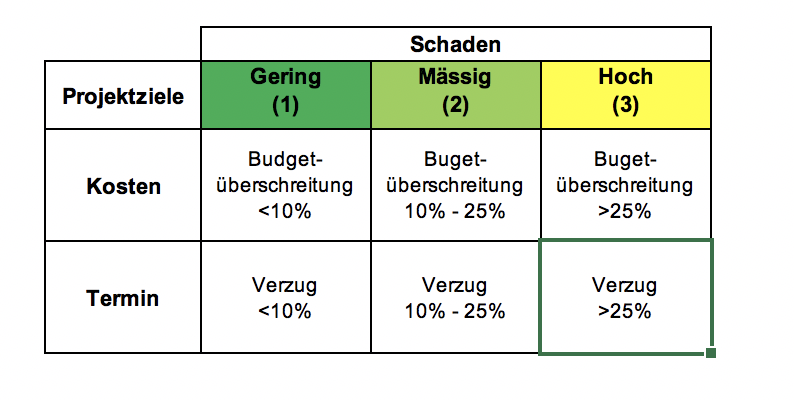
\includegraphics[width=14cm]{Schaden.png}
	\label{fig:Schaden}
\end{figure}

\begin{figure}[H]
	\centering
	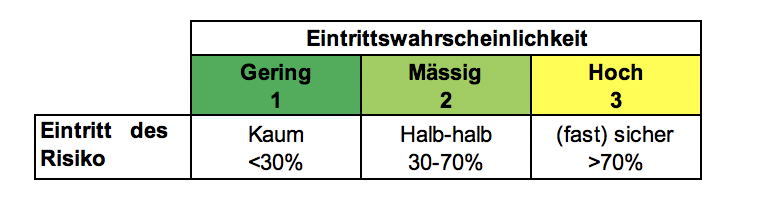
\includegraphics[width=14cm]{Eintrittswahrscheinlichkeit.png}
	\label{fig:Eintrittswahrscheinlichkeit}
\end{figure}
\newpage

\renewcommand{\arraystretch}{2}
\newcommand{\HY}{\hyphenpenalty = 25\exhyphenpenalty = 25}
%HY macht, dass Wörter innerhalb des Paragraphen in der Tabelle getrennt werden.
\definecolor{grau}{gray}{0.95}
\definecolor{weiss}{gray}{1}
\definecolor{schwarz}{gray}{0.1}
\definecolor{hgelb}{RGB}{255, 255, 0}
\definecolor{dgelb}{RGB}{231, 228, 17}
\definecolor{orange}{RGB}{253, 190, 0}
\definecolor{hgruen}{RGB}{150, 207, 57}
\definecolor{dgruen}{RGB}{116, 172, 56}
\begin{table}[H]
\tiny
\rotatebox{90}{
%\RaggedRight bewirkt, dass der Text nicht mehr im Blocksatz sondern Linksorientiert ist.
%\raggedRight funktioniert im Gegensatz zu RaggedRight nicht im Zusammenspiel mit HY
\begin{tabular}{c|>{\HY\RaggedRight}p{2.5cm}|>{\HY\RaggedRight}p{2.5cm}|>{\HY\RaggedRight}p{2.5cm}|c|c|c|>{\HY\RaggedRight}p{3cm}|>{\HY\RaggedRight}p{3cm}|c|c|c|c}
\multicolumn{7}{c}{\small \textbf{Risiko}}&\multicolumn{6}{c}{\small \textbf{Prävention}}\\
\textbf{Nr.}			&\textbf{Beschreibung}							&\textbf{Ursache	}																	&\textbf{Auswirkung}												&\textbf{Si}	&\textbf{Pi}	&\textbf{R}						&\textbf{Beschreibung}																					&\textbf{Auswirkung}																							&\textbf{Si'}	&\textbf{Pi'}	&\textbf{R'}				&\textbf{verantw.}\\
\hline
\textbf{A}			&Keine Verfügbarkeit von Komponenten				&Teile veraltet, ausverkauft															&Alternative muss gesucht werden									&2			&2			&\cellcolor{dgelb}4				&Im Voraus Alternativen einplanen																		&Falls eine Komponente nicht mehr verfügbar ist, kann schnell auf Alternative zurückgegriffen werden			&1				&2				&\cellcolor{hgruen}2		&PP\\
\rowcolor{grau}
\textbf{B}			&Ziele ändern sich								&Realisierung nicht möglich, Auftraggeber will etwas Neues							&Projekt kommt in grössere Dimensionen							&2			&2			&\cellcolor{dgelb}4				&Zielvorgaben werden zu Beginn klar definiert																&Keine unvorhergesehenen Änderungen treten auf																&1				&1				&\cellcolor{dgruen}1		&FI\\

\textbf{C}			&Projektmitglied fällt kurzfristig aus			&Krankheit, Terminkollision															&Zeitplan fällt zurück											&3			&1			&\cellcolor{hgelb}3				&Pufferzeiten einplanen, bereits bekannte Abwesenheit frühzeitig planen									&Zeitplan kann eingehalten werden																			&1				&1				&\cellcolor{dgruen}1		&CK\\
\rowcolor{grau}
\textbf{D}			&Projektmitglied fällt langfristig aus			&Studienabbruch, Unfall																&Verlust von Fachwissen und einer Fachkraft						&3			&1			&\cellcolor{hgelb}3				&Arbeit genau dokumentieren, Austausch unter den Projektmigliedern										&Fachwissen geht nicht verloren																				&1				&1				&\cellcolor{dgruen}1		&LB\\

\textbf{E}			&Projektmanager fällt kurzfristig aus			&Krankheit, Terminkollision															&Team arbeitet unkoordiniert, Arbeit wird nicht korrekt erledigt	&2			&2			&\cellcolor{dgelb}4				&Pufferzeiten einplanen, konsequent PM Stv. instruieren, bereits bekannte Abwesenheiten frühzeitig planen	&Bei PM-Ausfall kann reagiert werden																			&1				&1				&\cellcolor{dgruen}1		&PP\\
\rowcolor{grau}
\textbf{F}			&Projektmanager fällt langfristig aus			&Studienabbruch, Unfall																&Projekt kann nicht zu Ende geführt werden						&3			&1			&\cellcolor{hgelb}3				&PM Stv. instruieren																						&Projekt kann fortgeführt werden																				&2				&1				&\cellcolor{hgruen}2		&FI\\

\textbf{G}			&Projekt enthält zu anspruchsvolle Komponente		&Kompetenzen der Mitglieder wurden falsch eingeschätzt								&Aufgabe kann nicht zufriedenstellend ausgeführt werden			&2			&2			&\cellcolor{dgelb}4				&APs genau auf die einzelnen Mitglieder abstimmen															&Jeder ist im Stande, sein AP durchführen zu können															&2				&1				&\cellcolor{hgruen}2		&LB\\
\rowcolor{grau}
\textbf{H}			&Auftrag ist unklar definiert					&Lastenheft falsch, mehrdeutig														&Auftrag kann nicht zufriedenstellend ausgeführt werden			&3			&2			&\cellcolor{orange}6				&Vor Beginn alles genau definieren																		&Unklarheiten werden verhindert																				&3				&1				&\cellcolor{hgelb}3		&CK\\

\textbf{I}			&Strukturplan unvollständig						&Unerwartete APs kommen hinzu														&Zeitplan stimmt nicht mehr										&2			&2			&\cellcolor{dgelb}4				&Alle Projektmitglieder schauen den Projektpan an und ergänzen Fehlendes									&Vergessen von APs wird minimiert																			&2				&1				&\cellcolor{hgruen}2		&RF\\
\rowcolor{grau}
\textbf{J}			&Zeiten des APs sind zu knapp					&Schlechte Planung, schlechter Einsatz												&Zeiplan kommt durcheinander										&1			&3			&\cellcolor{hgelb}3				&Pufferzeiten einberechnen																				&Verspätunen werden verhindert																				&1				&1				&\cellcolor{dgruen}1		&MA\\

\textbf{K}			&Datenverlust									&Datenträger defekt, technische Probleme												&Alles muss erneut recherchiert werden, geschrieben werden		&3			&2			&\cellcolor{orange}6				&Backups regelmässig durchführen, auf mehreren Datenträger												&Der Datenverlust beschränkt sich auf die Zeit zum letzten Backup												&1				&1				&\cellcolor{dgruen}1		&LB\\
\rowcolor{grau}
\textbf{L}			&Soziale Spannung im Team						&Unfaire Arbeitsverteilung, Schlechte Qualität von einer Person, Meinungsdifferenz		&Motivation, Qualität, Arbeitsmoral sinken						&3			&2			&\cellcolor{orange}6				&Arbeitaufteilung bedacht angehen, Meinungsunterschiede besprechen										&Differenzen können stark reduziert werden																	&2				&1				&\cellcolor{hgruen}2		&RF\\
\end{tabular}
}
\end{table}

%\begin{figure}[H]
%	\centering
%	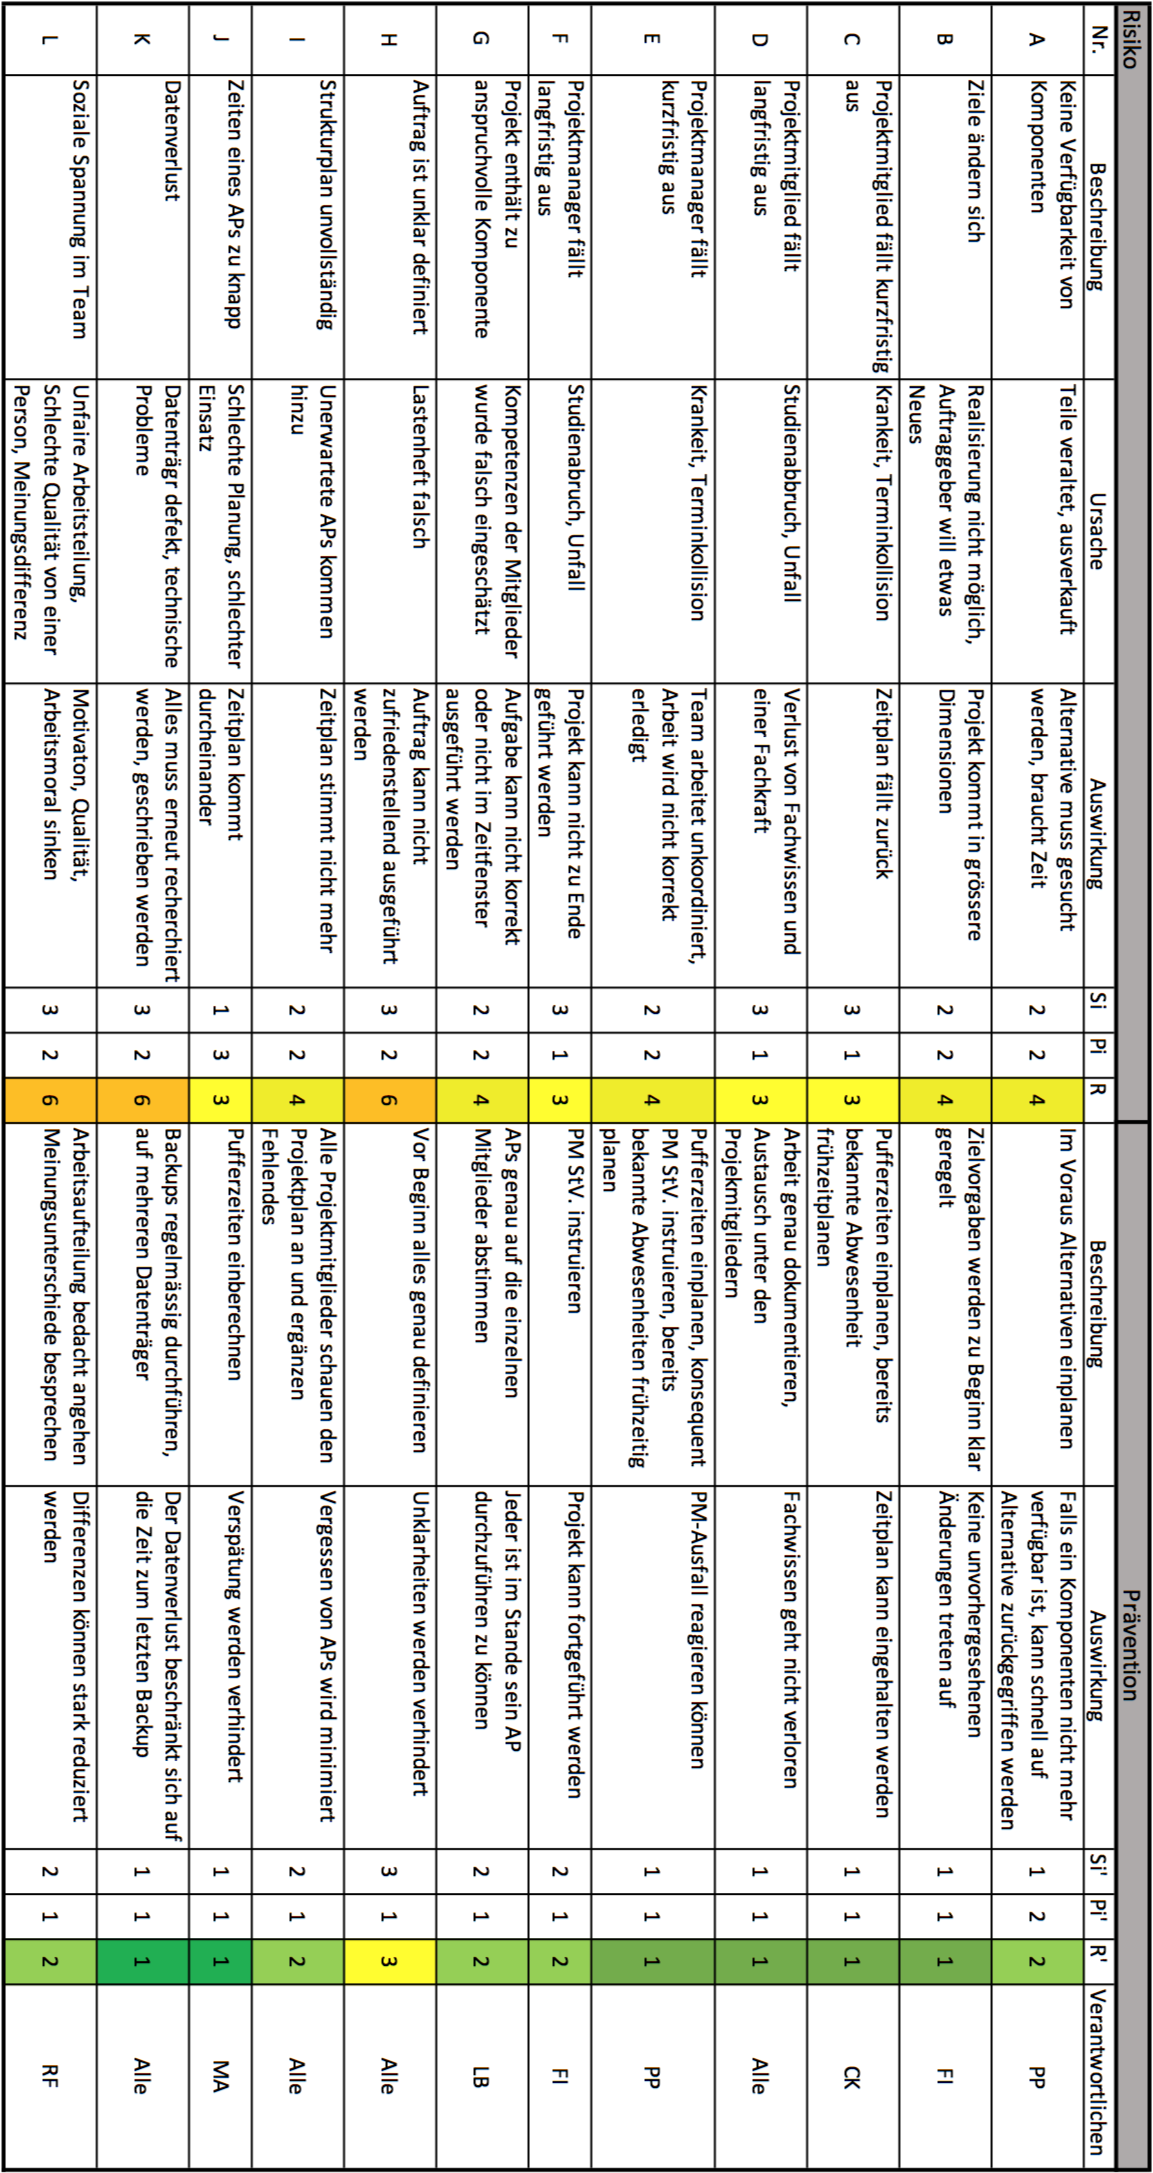
\includegraphics[angle= 180,width=12.5cm]{Risikoanalyse.png}
%	\label{fig:Risikoanalyse}
%\end{figure}

\newpage
\begin{figure}[H]
	\centering
	\includegraphics[width=14cm]{Risikotabelle}
	\label{fig:Tabelle}
\end{figure}
Um auf Risiken vorbereitet zu sein, haben wir obige Risikotabelle erstellt. In dieser listen wir die möglichen Gefahren auf und nennen Präventionsmassnahmen, um sowohl die Eintrittswahrscheinlichkeit(Pi), als auch die Auswirkungen(Si) zu minimieren.\\
Auf der folgenden Risikomap sind alle Gefahren mit und ohne Prävention graphisch dargestellt.

\begin{figure}[H]
	\centering
	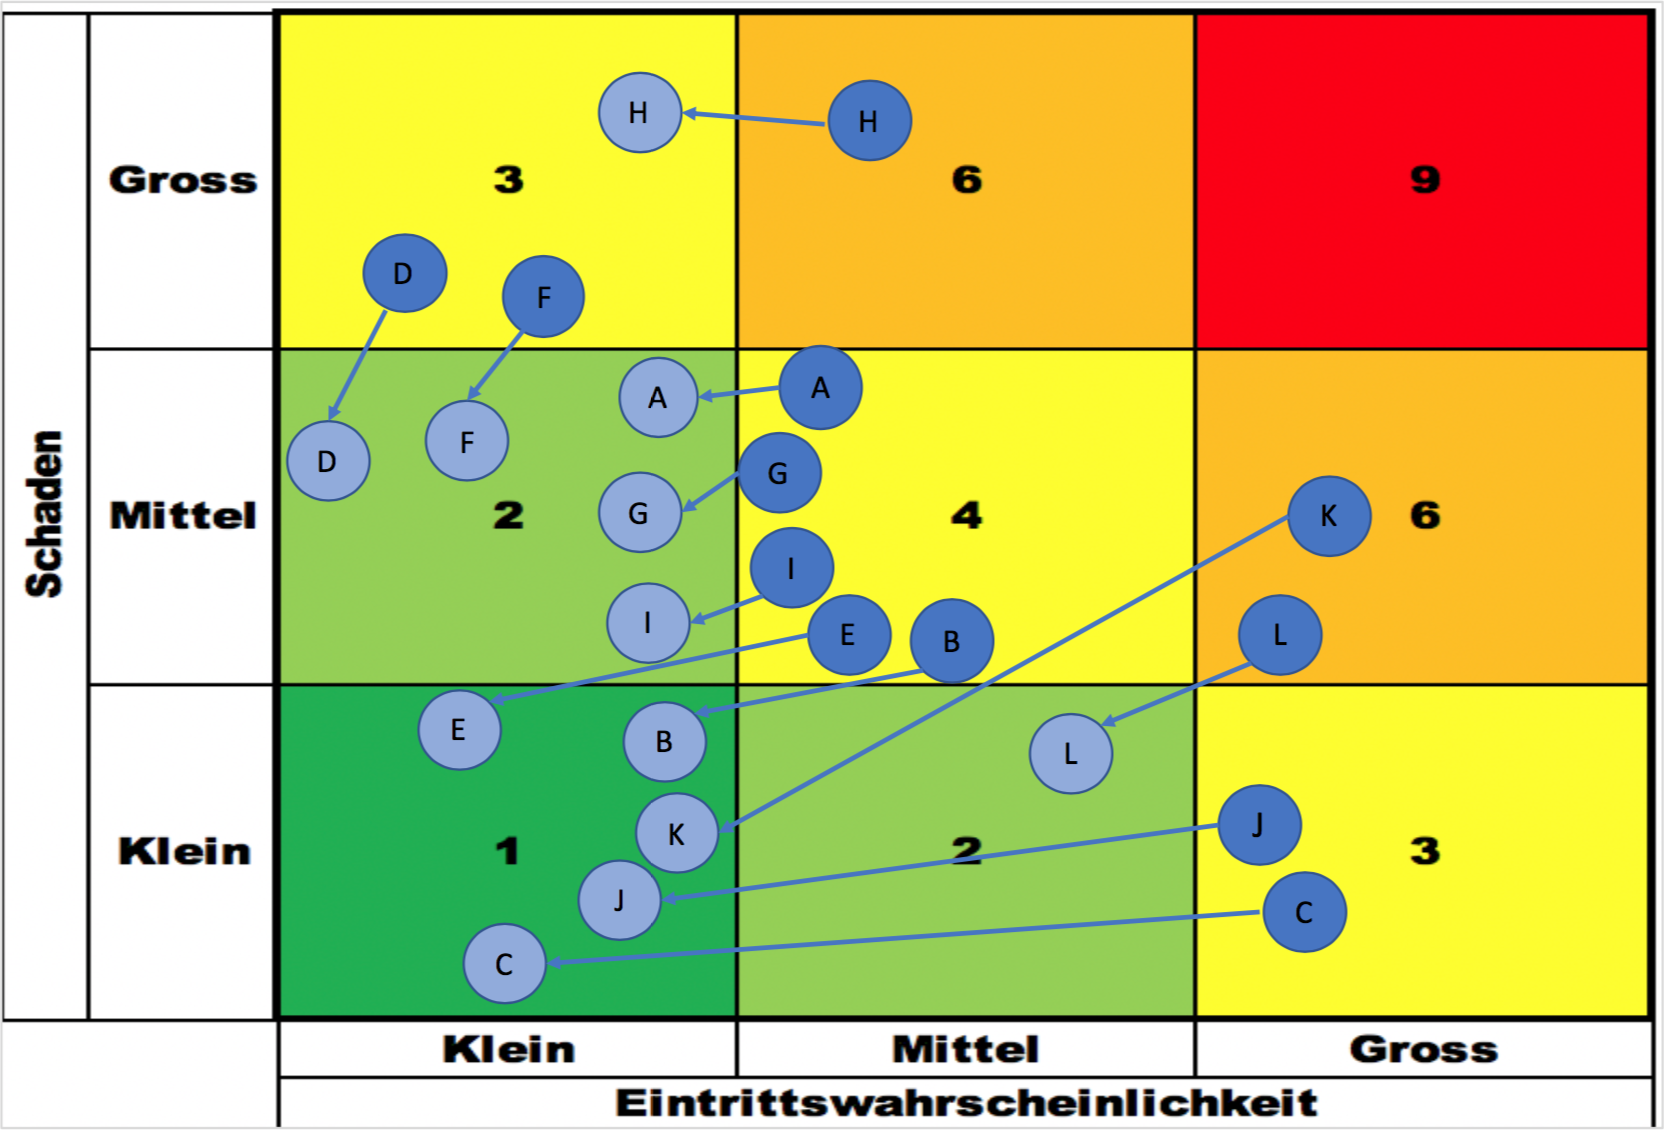
\includegraphics[width=14cm]{Risikotab.png}
	\label{fig:Risikodiagramm}
\end{figure}


A 	Keine Verfügbarkeit von Komponenten \newline 
B 	Ziele ändern sich\newline 
C 	Projektmitglied fällt kurzfristig aus\newline 
D	Projektmitglied fällt langfristig aus\newline 
E 	Projektmanager fällt kurzfristig aus\newline 
F 	Projektmanager fällt langfristig aus\newline 
G	Projekt enthält zu anspruchvolle Komponente\newline 
H	Auftrag ist unklar definiert\newline 
I	Strukturplan unvollständig\newline 
J	Zeiten eines APs zu knapp\newline 
K	Datenverlust\newline 
L	Soziale Spannung im Team\newline 
